\documentclass[twocolumn]{bmcart}
%\setlength{\footskip}{30pt}

%% Use the option review to obtain double line spacing
%% \documentclass[authoryear,preprint,review,12pt]{elsarticle}

%% Use the options 1p,twocolumn; 3p; 3p,twocolumn; 5p; or 5p,twocolumn
%% for a journal layout:
%% \documentclass[final,1p,times]{elsarticle}
%% \documentclass[final,1p,times,twocolumn]{elsarticle}
%% \documentclass[final,3p,times]{elsarticle}
%% \documentclass[final,3p,times,twocolumn]{elsarticle}
%% \documentclass[final,5p,times]{elsarticle}
%% \documentclass[final,5p,times,twocolumn]{elsarticle}

%% For including figures, graphicx.sty has been loaded in
%% elsarticle.cls. If you prefer to use the old commands
%% please give \usepackage{epsfig}

\usepackage[utf8]{inputenc}
%\usepackage[T1]{fontenc}
%\usepackage{lmodern}
%\usepackage{tgpagella}

% Extensive support for hypertext.
\usepackage[hidelinks,colorlinks=true]{hyperref}

% Easy access to the Lorem Ipsum dummy text.
\usepackage{lipsum}

% Pro­vides both fore­ground (text, rules, etc.) and back­ground colour man­age­ment.
%\usepackage{color}

% Driver-independent color extensions.
%\usepackage[x11names]{xcolor}

% Enhanced support for graphics.
\usepackage{graphicx}

% Produces figures which text can flow around.
\usepackage{wrapfig}

% Customising captions in floating environments.
%\usepackage{caption}

% Publication quality tables.
\usepackage{booktabs}

% Long tables.
\usepackage{longtable}

%% The amssymb package provides various useful mathematical symbols.
%\usepackage{amssymb}

%% The amsthm package provides extended theorem environments.
%\usepackage{amsthm}

%%%%%%%%%%%%%%%%%%%%%%%%%%%%%%%%%%%%%%%%%%%%%%%%%
%%                                             %%
%%  If you wish to display your graphics for   %%
%%  your own use using includegraphic or       %%
%%  includegraphics, then comment out the      %%
%%  following two lines of code.               %%
%%  NB: These line *must* be included when     %%
%%  submitting to BMC.                         %%
%%  All figure files must be submitted as      %%
%%  separate graphics through the BMC          %%
%%  submission process, not included in the    %%
%%  submitted article.                         %%
%%                                             %%
%%%%%%%%%%%%%%%%%%%%%%%%%%%%%%%%%%%%%%%%%%%%%%%%%

%\def\includegraphic{}
%\def\includegraphics{}

% Configure caption display.
%\captionsetup{margin=10pt,font=small,labelfont=bf,labelsep=period}

% Define where the images can be found.
\DeclareGraphicsExtensions{.pdf,.png,.jpg}
\graphicspath{{./images/}}

%%% Put your definitions there:
\startlocaldefs
\input{db-stats.inc}
\endlocaldefs

\begin{document}

% Configure hyperlink colors after document start to override possible
% documentclass defaults.
\hypersetup{
    citecolor=blue,
    filecolor=blue,
    linkcolor=blue,
    urlcolor=blue
}

\begin{frontmatter}

\begin{fmbox}
\dochead{Software}

%%%%%%%%%%%%%%%%%%%%%%%%%%%%%%%%%%%%%%%%%%%%%%
%%                                          %%
%% Enter the title of your article here     %%
%%                                          %%
%%%%%%%%%%%%%%%%%%%%%%%%%%%%%%%%%%%%%%%%%%%%%%

\title{Automated identification of slipper orchids using image analysis and artificial neural networks}

%%%%%%%%%%%%%%%%%%%%%%%%%%%%%%%%%%%%%%%%%%%%%%
%%                                          %%
%% Enter the authors here                   %%
%%                                          %%
%% Specify information, if available,       %%
%% in the form:                             %%
%%   <key>={<id1>,<id2>}                    %%
%%   <key>=                                 %%
%% Comment or delete the keys which are     %%
%% not used. Repeat \author command as much %%
%% as required.                             %%
%%                                          %%
%%%%%%%%%%%%%%%%%%%%%%%%%%%%%%%%%%%%%%%%%%%%%%

\author[
   addressref={nbc},
   %corref={},
   %noteref={},
   %email={}
]{\inits{S}\fnm{Serrano} \snm{Pereira}}
\author[
   addressref={nbc,hsl,lu},
   %corref={},
   noteref={n1},
   %email={}
]{\inits{B}\fnm{Barbara} \snm{Gravendeel}}
\author[
   addressref={nbc},
   %corref={},
   %noteref={},
   %email={}
]{\inits{P}\fnm{Patrick} \snm{Wijntjes}}
\author[
   addressref={nbc},
   %corref={},
   %noteref={},
   %email={}
]{\inits{R}\fnm{Rutger} \snm{Vos}}

% Dave Roberts co-author?

%%%%%%%%%%%%%%%%%%%%%%%%%%%%%%%%%%%%%%%%%%%%%%
%%                                          %%
%% Enter the authors' addresses here        %%
%%                                          %%
%% Repeat \address commands as much as      %%
%% required.                                %%
%%                                          %%
%%%%%%%%%%%%%%%%%%%%%%%%%%%%%%%%%%%%%%%%%%%%%%

\address[id=nbc]{
  \orgname{Naturalis Biodiversity Center}
  %\street{},
  %\postcode{}
  \city{Leiden},
  \cny{The Netherlands}
}

\address[id=hsl]{
  \orgname{University of Applied Sciences Leiden,}
  %\street{},
  %\postcode{}
  \city{Leiden},
  \cny{The Netherlands}
}

\address[id=lu]{
  \orgname{Institute Biology Leiden, Leiden University}
  %\street{},
  %\postcode{}
  \city{Leiden},
  \cny{The Netherlands}
}

%%%%%%%%%%%%%%%%%%%%%%%%%%%%%%%%%%%%%%%%%%%%%%
%%                                          %%
%% Enter short notes here                   %%
%%                                          %%
%% Short notes will be after addresses      %%
%% on first page.                           %%
%%                                          %%
%%%%%%%%%%%%%%%%%%%%%%%%%%%%%%%%%%%%%%%%%%%%%%

\begin{artnotes}
\note[id=n1]{Equal contributor} % note, connected to author
\end{artnotes}

% comment this for two column layout
%\end{fmbox}

%%%%%%%%%%%%%%%%%%%%%%%%%%%%%%%%%%%%%%%%%%%%%%
%%                                          %%
%% The Abstract begins here                 %%
%%                                          %%
%% Please refer to the Instructions for     %%
%% authors on http://www.biomedcentral.com  %%
%% and include the section headings         %%
%% accordingly for your article type.       %%
%%                                          %%
%%%%%%%%%%%%%%%%%%%%%%%%%%%%%%%%%%%%%%%%%%%%%%

\begin{abstractbox}

\begin{abstract}
A generic hierarchical identification system was developed for the automated identification of species by image recognition. The effectiveness of this system was assessed using photographs of orchids of the subfamily Cypripedioideae. Colour and shape features were extracted from single flower photos of {\SpeciesCount} orchid species. Generic image preprocessing, segmentation, and feature extraction algorithms were implemented to obtain morphometric data for the different orchid species. The identification system uses a hierarchy of artificial neural networks for pattern recognition and automated classification. The neural network hierarchy mirrors the taxonomic hierarchy of the Cypripedioideae, such that user-submitted photos could be assigned a genus, section, and species classification. The ability of the identification system to correctly identify user-submitted photos varied depending on the photo quality, the number of species included for training, and the desired taxonomic level for identification. High quality photos were scarce for some taxa and were under-represented in the training set, resulting in imbalanced network training. The simple colour features used for training were not sufficient to reliably identify photos to the correct section and species, and more specialised feature extraction algorithms need to be developed to improve accuracy. The outcomes of this project include an open source library of feature extraction libraries called ImgPheno, a collection of scripts for neural network training called NBClassify, and a web-interface for NBClassify called OrchiD for identification of user-submitted images.
\end{abstract}

%%%%%%%%%%%%%%%%%%%%%%%%%%%%%%%%%%%%%%%%%%%%%%
%%                                          %%
%% The keywords begin here                  %%
%%                                          %%
%% Put each keyword in separate \kwd{}.     %%
%%                                          %%
%%%%%%%%%%%%%%%%%%%%%%%%%%%%%%%%%%%%%%%%%%%%%%

\begin{keyword}
    \kwd{Cypripedioideae}
    \kwd{feature extraction}
    \kwd{identification}
    \kwd{image analysis}
    \kwd{neural networks}
    \kwd{orchids}
    \kwd{pattern recognition}
    \kwd{taxonomy}
\end{keyword}

% MSC classifications codes, if any
%\begin{keyword}[class=AMS]
%\kwd[Primary ]{}
%\kwd{}
%\kwd[; secondary ]{}
%\end{keyword}

\end{abstractbox}

% uncomment this for twcolumn layout
\end{fmbox}

\end{frontmatter}

%%%%%%%%%%%%%%%%%%%%%%%%%%%%%%%%%%%%%%%%%%%%%%
%%                                          %%
%% The Main Body begins here                %%
%%                                          %%
%% Please refer to the instructions for     %%
%% authors on:                              %%
%% http://www.biomedcentral.com/info/authors%%
%% and include the section headings         %%
%% accordingly for your article type.       %%
%%                                          %%
%% See the Results and Discussion section   %%
%% for details on how to create sub-sections%%
%%                                          %%
%% use \cite{...} to cite references        %%
%%  \cite{koon} and                         %%
%%  \cite{oreg,khar,zvai,xjon,schn,pond}    %%
%%  \nocite{smith,marg,hunn,advi,koha,mouse}%%
%%                                          %%
%%%%%%%%%%%%%%%%%%%%%%%%%%%%%%%%%%%%%%%%%%%%%%

\section{Introduction}
\label{sect:introduction}

Correct taxonomic identification of life on earth is for different reasons of great importance. Considering the case of the Cypripedioideae, a horticultural popular group of orchids species and from which many species are highly endangered in the wild, correct taxonomic identification is necessary in order to protect them. Expert taxonomic identification is rare and costly, so alternative methods for taxonomic identification that are both cheap and accurate enough would be of great value. Ongoing advances in computer vision and machine learning has lead to the development of numerous semi- and fully automated species identification systems. Such systems have been successful in the identification of plant species \cite{Arinkin2014, Nilsback2008, Sanz2013}, phytoplankton \cite{Boddy1994}, diatom frustules \cite{Kloster2014}, and insects \cite{Weeks1999,Kang2012}, amongst others. Artificial Neural Networks (ANNs) in particular have become an increasingly popular choice in automated image classification systems \cite{Weeks1997}. They provide a powerful tool for pattern recognition and machine learning.

\section{Materials and methods}
\label{sect:methods}

% Used social media (crowd sourcing) for the collection of images.

\subsection{Reference photo collection}

A collection of reference photos was compiled by searching the internet for images, mostly through Google Image searches. The correct genus, section, and species for each image was verified by specialists and referenced to the literature \cite{Cribb1998, Pridgeon1999, Frosch2012} and phylogenetic reconstructions based on molecular analyses \cite{Li2011, Chochai2012}. Every photo was subsequently uploaded to an account on the online image hosting service Flickr (\url{https://www.flickr.com}). On Flickr, each image was annotated with standardized tags in the formats \texttt{genus:name}, \texttt{section:name}, and \texttt{species:name}. A custom Python script utilizing the Flickr API was used to download the entire image collection with metadata from the Flickr account to a local computer, where images are stored in a directory hierarchy and image annotations are stored in a database (\ref{sect:meta-database}).

\subsection{Image feature extraction}

The decision was made to develop a generic open-source library of feature extraction methods in an attempt to create a centralized collection of the many image feature extraction algorithms developed over the years. A Python package called ImgPheno (\url{https://github.com/naturalis/imgpheno}) was developed as a result, which is a collection of several image feature extraction methods. It is implemented by a collection of proof-of-concept Python scripts (\url{https://github.com/naturalis/nbclassify}) for image feature extraction and neural network training. The source code of the Python packages are released under the MIT license so that anyone can modify and use this work without restriction. The scripts make extensive use of OpenCV \cite{Pulli2012} for computer vision functionality, NumPy \cite{VanderWalt2011} for array manipulation functionality, and of scikit-learn \cite{Pedregosa2011} for data manipulation functionality. The NBClassify package contains a Python script that automates image feature extraction and neural network training. Configurations are kept in a separate configuration file so that neural network training can easily be reproduced. For feature extraction such configurations include image preprocessing (scaling, colour correction, foreground segmentation), features to be extracted, data format, and a classification hierarchy definition for generating training data for training a neural network hierarchy.

As part of the feature extraction workflow, each image is first scaled down if the image exceeds a predefined maximum dimension. This is followed by foreground segmentation, where the background pixels are removed, ideally keeping only the pixels that make up the flower. Foreground segmentation is done using the GrabCut segmentation algorithm \cite{Rother2004}, which uses an iterative approach. The region of interest (ROI) for the first iteration is set to the entire image and is shrank a fixed number of pixels to get a margin around the ROI containing obvious background pixels (figure \ref{fig:grabcut-output}). Images must therefore be reasonably standardized such that the flower is somewhere in the centre of the image and there must also be good contrast between the flower and the background, as to keep segmentation errors to a minimum. Subsequent iterations further classify pixels inside the ROI as foreground or background until the maximum number of iterations is reached. Contours are then obtained from the resulting binary mask. If multiple contours are found, only the largest contour is used to select the foreground pixels for downstream feature extraction.

\begin{figure*}[t]
    \centering
    \minipage{\textwidth}
        \includegraphics[width=0.48\linewidth]{grabcut_output_roi.png}
        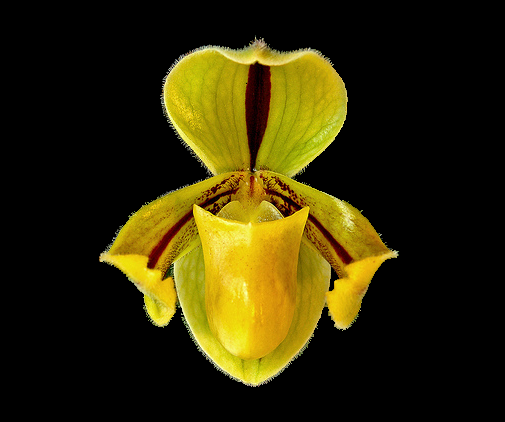
\includegraphics[width=0.48\linewidth]{grabcut_output.png}
    \endminipage
    \caption{Foreground segmentation with the GrabCut algorithm. The image on the left displays how the initial region of interest is set during automated feature extraction. Photo of \textit{Paphiopedilum druryi} by Peter Tremain.}
    \label{fig:grabcut-output}
\end{figure*}

BGR colour data were extracted and used as features for training the neural networks. This was done by calculating the up-right bounding square for the main contour, dividing the square into $N$ equal horizontal and vertical sections (bins), and calculating the mean blue, green, and red colour intensity for each bin (figure~\ref{fig:bgr-means-sections}). Plotting the mean BGR colour intensities shows that this feature captures some information about flower shape as well (figure~\ref{fig:bgr-means-plots}).

\begin{figure}[h]
    \centering
    \includegraphics[width=0.46\textwidth]{bgr_means_sections.png}
    \caption{The second horizontal and vertical bin ($N~=~20$) is highlighted in a foreground segmented image of \textit{P.~druryi}.}
    \label{fig:bgr-means-sections}
\end{figure}

\begin{figure*}[t]
    \centering
    \includegraphics[width=\textwidth]{bgr_means_plots.pdf}
    \caption{Plots of the mean BGR colour intensities for an image of \textit{P. druryi}. The plots display the mean intensities for the horizontal and vertical bins respectively.}
    \label{fig:bgr-means-plots}
\end{figure*}

\subsection{Neural network training}

Artificial Neural Network (ANN) training was implemented with the Fast Artificial Neural Network Library (FANN) by \cite{Nissen2003}. The same Python script used for generating the training data was used for training the neural networks for a given classification hierarchy. The classification hierarchy is defined in a configurations file and is defined as a list of levels which tells the script the path to follow during training and classification (i.e. $genus \rightarrow section \rightarrow species$). Different features and training parameters can be set at each level in the classification hierarchy, which the script then uses to generate training data and train the neural networks for hierarchical classification.

\subsection{Cross-validation}

Stratified k-folds cross-validation was performed to estimate the accuracy of the classifiers. Genus, section, species combinations were used as the classes for the cross-validations. The number of folds was set to 4 ($k=4$) to include only those taxa for which at least 4 photos were present. Cross-validation was also performed with 10 folds, only including the species represented by at least 10 photos.

Principal components analysis (PCA) was performed on the training data to assess the suitability of the features to identify the photos by genus, section, and species.

\section{Results}
\label{sect:results}

\subsection{Reference photo collection}

In total {\PhotoCount} photos for {\SpeciesCount} species were collected (table~\ref{tbl:photo-counts}). The collection contains photos for the genera \textit{Cypripedium}, \textit{Mexipedium}, \textit{Paphiopedilum}, \textit{Phragmipedium}, and \textit{Selenipedium}. With the number of photos for the five genera ranging from just 4 for the genus \textit{Selenipedium} to 888 for \textit{Paphiopedilum}, the collection is highly unbalanced.

\begin{table}[h]\footnotesize
    \caption{The number of photos collected per genus, as well as the number of sections and species per genus represented by the photo collection.}
    \begin{center}
    \begin{tabular}{llll}
    \toprule
    \textbf{Genus} & \textbf{Section} & \textbf{Species} & \textbf{Photos} \\
    \midrule
    \input{table-taxa-summary.inc}
    \bottomrule
    \end{tabular}
    \end{center}
    \label{tbl:photo-counts}
\end{table}

\subsection{Image feature extraction}

Several image feature extraction methods were implemented in the ImgPheno library.

\begin{table}[h]\footnotesize
    \caption{Selection of ImgPheno methods.}
    \begin{center}
    \begin{tabular}{lp{4cm}}
    \toprule
    \textbf{Method} & \textbf{Description} \\
    \midrule
    \verb/color_bgr_means/ & Returns the histograms for BGR images along X and Y axis. \\
    \bottomrule
    \end{tabular}
    \end{center}
    \label{tbl:imgpheno-methods}
\end{table}

\subsection{Cross-validation}

Stratified k-folds cross-validation was performed to estimate the accuracy of the classifiers. The accuracy for genus classification was 75\%, but accuracy drops dramatically as section (52\%) and species (48\%) are also included in the classification (table~\ref{tbl:x-validation-results}). With 10 folds and including only those species for which at least 10 photos are collected, results in slightly better accuracies (table~\ref{tbl:x-validation-results}), but this can probably be attributed to the reduced number of sections and species.

\begin{table}[h]\footnotesize
    \caption{Results for stratified k-fold cross-validations. Cross-validation was performed on three taxonomic ranks: genus, section, and species. The results for genus/section and genus/section/species combine the results from their respective ranks.}
    \begin{center}
    \begin{tabular}{lp{1.5cm}p{1.5cm}}
    \toprule
    \textbf{Classification} & \textbf{Accuracy (k=4)} & \textbf{Accuracy (k=10)} \\
    \midrule
    genus                   & 75\%    & 81\% \\
    section                 & 52\%    & 60\% \\
    species                 & 48\%    & 56\% \\
    genus/section           & 41\%    & 49\% \\
    genus/section/species   & 20\%    & 27\% \\
    \bottomrule
    \end{tabular}
    \end{center}
    \label{tbl:x-validation-results}
\end{table}

Principal components analysis (PCA) with orthogonal rotation (varimax) was conducted on training training data for genus classification containing -1 to 1 scaled mean colour intensities for the BGR colour space with 20 horizontal and vertical bins, which translates to 120 features. The Kaiser-Meyer-Olkin measure verified the sampling adequacy for the analysis with an overall Measure of Sampling Adequacy (MSA) of 0.92, and all MSA values for individual items were >0.76, which is well above the acceptable limit of 0.5. Bartlett's test of sphericity $\chi^2 (7140) = 452642$, $p = 0$, indicated that correlations between items were sufficiently large for PCA. An initial PCA was run to obtain eigenvalues for each component in the data. The scree plot constructed from the eigenvalues showed inflexion that would justify retaining 3 components (explaining 65\% of the variance). Given the large sample size (N = 1134) and the convergence of the scree plot, 3 components were retained in the final analysis. The same PCA workflow was repeated for training data for section classification within the genus Paphiopedilum, and for species classification within the section Parvisepalum of genus Paphiopedilum. Figure~\ref{fig:pca-plots} shows the scatter plots for the principal components.

\section{Conclusions and discussion}
\label{sect:conclusion}

In an effort the normalize images prior to feature extraction, some colour image enhancement methods developed by \cite{Naik2003} were implemented. Most images used were already of good quality, and performing hue-preserving linear transformation with maximum contrast often did not result in an enhanced image, and thus colour enhancement using this method did not result in improved identification accuracy. Several feature extraction method were implemented in the ImgPheno package, including methods for obtaining image moments based shape characteristics, methods for getting contour outline characteristics (e.g. convex area, eccentricity, equivalent diameter, extent, orientation, perimeter, solidity), specialised shape description methods, and methods for obtaining colour data. This study builds on a simple features extraction method for obtaining colour data, \verb/color_bgr_means/.

As opposed to simply using overall colour data as described in this study, image feature extraction methods should also be developed for extracting specific morphological characters to improve accuracy with hierarchical classification. Developing such specialized features extraction methods is not an easy task however. Many different specialized image feature extraction methods have been developed, and it would be desirable to have these combined in a freely available library, as was attempted in this study. And since multiple morphological characters are usually considered during species identification, multiple features or characters can be represented by the feature data. Identification accuracy can further be improved by means of neural network ensembles, the usage of multiple neural networks to make classifications \cite{Hansen1990}. The identification system presented here does use multiple neural networks for the identification of an image, but these cannot be considered neural networks ensembles because only one neural network is used for each level within the hierarchical classification (i.e. one neural network is used for genus, section, and species separately). The output codes used for training the neural networks as implemented in this study is another aspect that could be improved. The implementation presented here uses the simplest possible output codes for training, but the usage of more sophisticated error codes could improve neural network training and therefore identification accuracy \cite{Dietterich1995}.

% Need more and better photo material.
% Better feature extraction methods.

%%%%%%%%%%%%%%%%%%%%%%%%%%%%%%%%%%%%%%%%%%%%%%
%%                                          %%
%% Backmatter begins here                   %%
%%                                          %%
%%%%%%%%%%%%%%%%%%%%%%%%%%%%%%%%%%%%%%%%%%%%%%

\begin{backmatter}

\section*{Acknowledgements}

% De namen van alle fotografen in de format J.H. Simpson.

\lipsum[1]

%%%%%%%%%%%%%%%%%%%%%%%%%%%%%%%%%%%%%%%%%%%%%%%%%%%%%%%%%%%%%
%%                  The Bibliography                       %%
%%                                                         %%
%%  Bmc_mathpys.bst  will be used to                       %%
%%  create a .BBL file for submission.                     %%
%%  After submission of the .TEX file,                     %%
%%  you will be prompted to submit your .BBL file.         %%
%%                                                         %%
%%                                                         %%
%%  Note that the displayed Bibliography will not          %%
%%  necessarily be rendered by Latex exactly as specified  %%
%%  in the online Instructions for Authors.                %%
%%                                                         %%
%%%%%%%%%%%%%%%%%%%%%%%%%%%%%%%%%%%%%%%%%%%%%%%%%%%%%%%%%%%%%

% if your bibliography is in bibtex format, use those commands:
\bibliographystyle{bmc-mathphys} % Style BST file
%\bibliographystyle{apa}
%\biboptions{authoryear}

% or include bibliography directly:
% \begin{thebibliography}
% \bibitem{b1}
% \end{thebibliography}

\bibliography{references}

%% The Appendices part is started with the command \appendix;
%% appendix sections are then done as normal sections
\appendix
\onecolumn

\section{Metadata database}
\label{sect:meta-database}

\begin{figure*}[!h]
    \centering
    \includegraphics[width=\textwidth]{meta_database_diagram.pdf}
    \caption{Diagram of the metadata database used for storing taxonomic information for a collection of reference photos.}
    \label{fig:meta-database}
\end{figure*}

\section{Reference photo collection}
\label{sect:reference-photo-collection}

\begin{footnotesize}
\begin{longtable}{llllll}
    \caption{Taxa represented by the reference photo collection and the number of photos for each species.}
    \label{tbl:taxa-stats}
    \endfirsthead
        \caption*{\textbf{Table \ref{tbl:taxa-stats}.} (continued)}
        \\\textbf{Taxa} & \textbf{Photos} \\
        \midrule
    \endhead
        %\midrule
        \caption*{\footnotesize\textit{(continued on next page)}}
    \endfoot
        \bottomrule
    \endlastfoot

    \toprule
    \textbf{Taxa} & \textbf{Photos} \\
    \midrule
    \input{table-taxa.inc}
\end{longtable}
\end{footnotesize}

\clearpage
\section{Scatter plots for principal components analyses}
\label{sect:pca-plots}

\begin{figure}[!h]
    \minipage{\textwidth}
        \includegraphics[width=0.5\linewidth]{genus_pca_plot.pdf}
        \includegraphics[width=0.5\linewidth]{Cypripedium_section_pca_plot.pdf}
    \endminipage
    \par\vfill
    \minipage{\textwidth}
        \includegraphics[width=0.5\linewidth]{Paphiopedilum_section_pca_plot.pdf}
        \includegraphics[width=0.5\linewidth]{Paphiopedilum_Parvisepalum_species_pca_plot.pdf}
    \endminipage
    \caption{Scatter plots for the principal components analysis results. PCA was conducted on training data for genus classification, \textit{Cypripedium} section classification, \textit{Paphiopedilum} section classification, and \textit{Paphiopedilum} section \textit{Parvisepalum} species classification. For all plots the first principal component (PC1) was plotted against the second (PC2).}
    \label{fig:pca-plots}
\end{figure}

\end{backmatter}
\end{document}
